\documentclass[a0paper,12pt]{article}
\usepackage[landscape,top=5cm,bottom=3cm,right=5cm,left=5cm]{geometry}
\usepackage{graphicx}
\usepackage{standalone}
\usepackage{amsmath}
\usepackage[T1]{fontenc}
\usepackage{lmodern}
\usepackage{tikz}
\usepackage{tikzscale}
\usepackage{enumitem}
\usetikzlibrary{shapes,arrows}
\usetikzlibrary{arrows.spaced}
\usetikzlibrary{decorations.text}
\usetikzlibrary{spy,calc}
\usetikzlibrary{shapes.arrows}

\usepackage{color}
\usepackage{moresize}
\usepackage{lipsum} % dummy text
\usepackage{multicol}

\pgfdeclarelayer{background}
\pgfdeclarelayer{layer1}
\pgfdeclarelayer{layer2}
\pgfdeclarelayer{layer3}
\pgfdeclarelayer{foreground}

\newenvironment{Figure}
  {\par\medskip\noindent\minipage{\linewidth}}
  {\endminipage\par\medskip}

% This macro creates header.
\newcommand{\HEADING}[1]
{
    %\includegraphics[scale=0.35]{./images/heading.png}
    \MOOSELOGO
    \fontsize{2.5cm}{1cm}\selectfont \textcolor{red}{#1}
    \vspace{0.5cm}
}

\newcommand{\SECTION}[1]
{
    {\fontsize{2cm}{1.5cm}\selectfont \textsc{\textcolor{blue}{#1}}\par}
}

\newcommand{\CAPTION}[1]
{
    {\fontsize{1cm}{1cm}\fontfamily{\sfdefault}\selectfont {\textcolor{black}{#1}}\par}
}

\newcommand{\TEXT}[1]
{
   { \fontsize{1.5cm}{1.5cm}\fontfamily{\sfdefault}\selectfont {#1}\par }
}

\newcommand{\ITEM}[1]
{
    {\fontsize{1.2cm}{1.2cm}\fontfamily{\sfdefault}\selectfont {#1}\par }
}

\newcommand{\MOOSE}[0]{\textsc{\textcolor{red}{MOOSE}}}

\newcommand{\MOOSELOGO}[0]{
    \tikz \node[inner sep=1mm] {\includegraphics[scale=0.6]{./images/moose_logo_tiny.png}}; 
}

\tikzset{
  every overlay node/.style={
    draw=black,fill=white,rounded corners,anchor=north west,
  },
}
% Usage:
% \tikzoverlay at (-1cm,-5cm) {content};
% or
% \tikzoverlay[text width=5cm] at (-1cm,-5cm) {content};
\def\tikzoverlay{%
   \tikz[baseline,overlay]\node[draw=white,every overlay node]
}%

\begin{document}

\begin{tikzpicture}[remember picture,overlay] 
    \node[opacity=1.0] (background) at (current page.center) {
        
\includegraphics[width=\paperwidth,height=\paperheight]{./background/background.jpg}
    };
\end{tikzpicture}


\begin{minipage}{\textwidth}
    \centering
    \fontsize{4cm}{1em}\selectfont \textcolor{red}{Modelling Memory Across Scale}
    \\
    \fontsize{1.5cm}{1em}\selectfont Aditya Gilra, Aviral Goel, Dilawar Singh,
    Harsha Rani, Sahil Moza, Subhasis Ray, Upinder Bhalla
\end{minipage}

%% Three columns
\vspace{5cm}
\setlength{\columnsep}{6cm}
\begin{multicols}{3}
    
%%%%%%%%%%%% Column 1
\begin{Figure}
    \HEADING{Why Multiscale?}

    \begin{Figure}
        %\begin{tikzpicture}[]
    \LARGE
    \def\lengthScaleFactor{1.6}
    \def\timeScaleFactor{1.6}

    \newcommand\scaleNode[1]{
        (0, #1*\timeScaleFactor)
    }

    \coordinate (sizeRoot) at (0, 1);
    \coordinate (sizeends) at (0,-1+11*\lengthScaleFactor);
    \coordinate (timeRoot) at (1,0);
    \coordinate (timeends) at (1+11*\timeScaleFactor, 0);


    \draw[-fast cap, blue!20!white, line width=6ex]  (timeRoot) to[] (timeends);
    \draw[-fast cap, blue!20!white, line width=6ex]  (sizeRoot) to[] (sizeends);


    \node[] (nm) at (0,1) {$10^{-9}m$};
    \node[] (um) at (0,5) {$10^{-6}m$};
    \node[] (mm) at (0,9) {$10^{-3}m$};
    \node[] (m) at (0,13) {$10^{-0}m$};

    \node[] (us) at (1.5,0) {$\mu$ sec};
    \node[] (ms) at (4.5,0) {$m$ sec};
    \node[] (s) at (7.5,0) {sec};
    \node[] (hrs) at (10.5, 0) {hours};
    \node[] (days) at (13.5, 0) {days};

    %% Distance between images and y-axis.
    \def\shifty{-3.0cm}

    \node[] (n1) at ([xshift=\shifty,yshift=0cm]nm) {
        \includegraphics[width=0.1\textwidth]{images/8tim_TIM_barrel.png}
    };

    \node[] (n2) at ([xshift=\shifty,yshift=0cm]um) {
        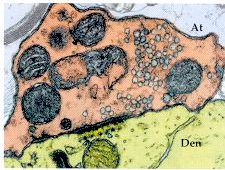
\includegraphics[width=0.1\textwidth]{images/dendrite.png}
    };

    \node[] (n3) at ([xshift=\shifty,yshift=-1cm]mm) {
        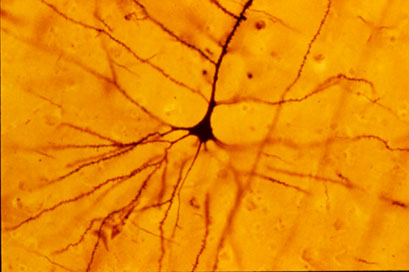
\includegraphics[width=0.1\textwidth]{images/GolgiStainedPyramidalCell.jpg}
    };

    \node[] (n4) at ([xshift=\shifty,yshift=1cm]mm) {
        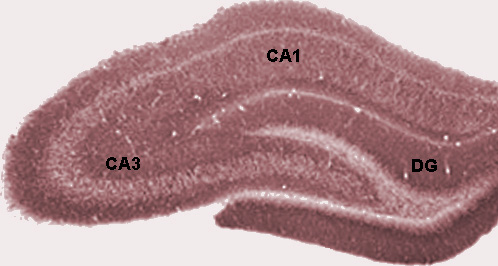
\includegraphics[width=0.1\textwidth]{images/HippocampalRegions.jpg}
    };

    \node[] (n5) at ([xshift=\shifty,yshift=-1.0cm]m) {
        \includegraphics[width=0.1\textwidth]{images/brain.png}
    };

    \node[opacity=0.5, rectangle, minimum width=12cm, minimum height=7.0cm,
    fill=blue!20, rounded corners] (chemical) at (9.0,4.5) {};

    \node[] (caption) at ([yshift=-1cm]chemical.north) {\LARGE Chemical};

    \node[opacity=0.5, rectangle, minimum width=4cm, minimum height=7cm, fill=red!20, rounded corners] 
    (electrical) at (4.0, 11.0) {};

    \node[] at (electrical.center) {\LARGE Electrical};


    % Put chemical network here
    \node[] (network) at (7.0,4.0) {
        \includegraphics[width=5cm]{images/chemical_reactions.png}
    };

    \node[] (chromosome) at (11.0,6.0) {
        
\includegraphics[width=5cm]{images/chromosome.png}
    };

    \node[fill=red!1] (text) at ([xshift=5cm]electrical.east) {
        \begin{minipage}{0.3\textwidth}
            \large
            \begin{itemize}
                \item $10^{11}$ cells, $10^{15}$ synapses, $10000$? reactions per synapse
                \item Electrical events: $< 1$ ms,  Chemical events: $1\;
                    \text{sec} \rightarrow 1000\; \text{sec}$
            \item Structural events: $100\; \text{sec} \rightarrow \text{months}$
        \item Lifetime of a protein: days, a neuron: 100 years, a memory: 100 years
    \end{itemize}
\end{minipage}
        };
    \end{tikzpicture} %



        \begin{itemize}
            \item \TEXT{Memory and plasticity involve brain mechanisms from molecular scale
                    to enormous networks.}

            \item \TEXT{We have developed \textcolor{red}{\textsc{MOOSE}}
                    the Multiscale Object Oriented Simulation
                    Environment, to model plasticity across scales.}

        \end{itemize}

     \begin{tikzpicture}[
        spy using outlines={circle
            , magnification=10, connect spies
        }
                 ]
         \centering
         \node [] (image) at (0,-1) {
             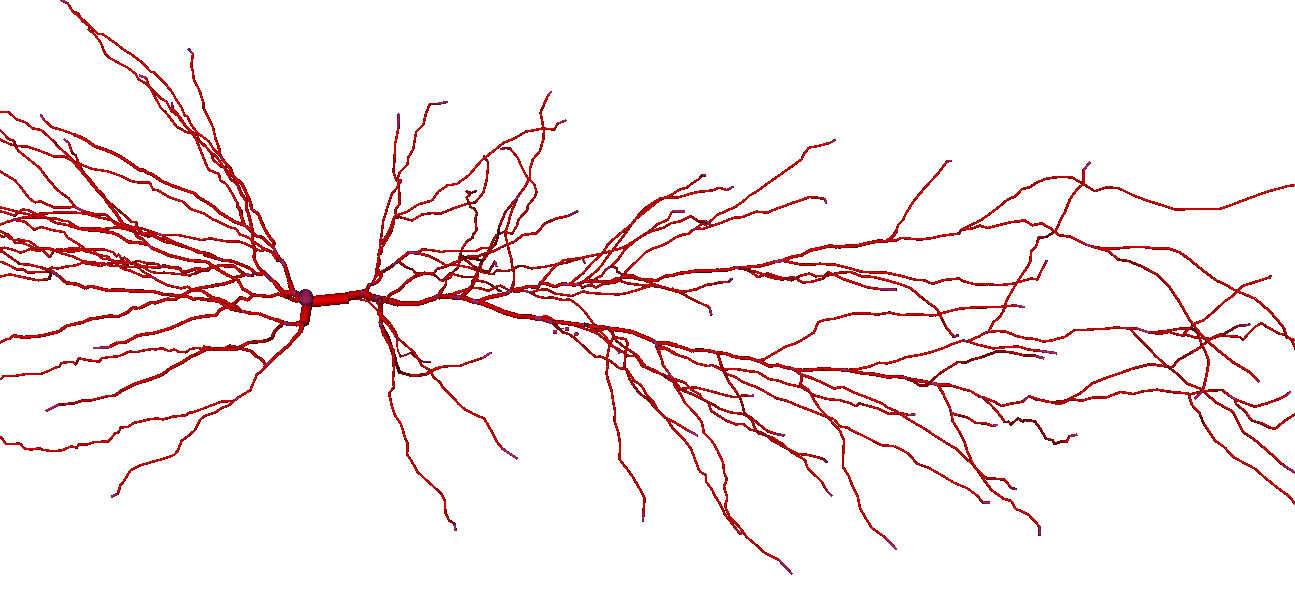
\includegraphics[scale=0.2,angle=-30]{./images/ca1_neuron.png}
         };

         \foreach \i in {-3,...,3}
         \foreach \j in {-3,...,3}
         {
             \node[fill=blue!40,opacity=0.3,thin,inner sep=0pt, minimum size=3mm,circle] (n\i\j) at (\i, \j) {};
         };

         \spy[blue, size=3cm] on (1.65, -1.5) in node[left] at (7,3);
         \node[below=4cm,text width=0.3\textwidth] {\CAPTION{A single neuron is
                 embedded in lattice of neural network}};

         %% Cool. Now create a 3d compartment model here.
         \begin{scope}[xshift=11cm, yshift=3cm
             , compartment/.style={cylinder
                 , draw
                 , cylinder uses custom fill
                 , cylinder end fill = red!35
                 , cylinder body fill = red!40
                 , inner sep = 3mm
                 , minimum height = 1cm
                 , minimum width = 1cm 
             }
             , spine/.style={cylinder 
                 , fill = blue!20
                 , inner sep=1mm
                 , minimum height=1mm
                 , minimum width=3mm
             }
             , branch/.style={cylinder
                 , draw
                 , cylinder uses custom fill
                 , cylinder end fill = red!35
                 , cylinder body fill = red!40
                 , minimum height = 1.5cm
                 , minimum width = 0.5cm
                 , inner sep = 1mm
             }
             ]

             \node[compartment] (c1) {};
             \node[compartment] (c2) at (c1.east) {};
             \node[compartment] (c3) at (c2.east) {};

             \node[branch,rotate=45] (b1) at ([xshift=4mm,yshift=2mm]c3.before top) {};
             \node[branch,rotate=-45] (b2) at ([xshift=1mm, yshift=-7mm]c3.base east) {};

             % Spines
             \node[spine, inner sep=1mm, rotate=135] (s11) at (b1.north east) {};
             \node[spine, inner sep=1mm, rotate=135] (s12) at ([xshift=3mm]b1.south east) {};

             \node[spine, inner sep=1mm, rotate=45] (s21) at (b2.north east) {};
             \node[spine, inner sep=1mm, rotate=45] (s22) at ([xshift=-3mm]b2.south east) {};

         \end{scope}

         %% Scope to draw chemisty 
         \begin{scope}

             \node[] (chemical) at ([yshift=-5.5cm]c2.south) {
                 \includegraphics[width=0.35\textwidth, trim=5mm 5mm 5mm 5mm, clip]{./images/chemical_reactions.png}
             };

             %%  
             \node [above] (chemicallabel) at ([yshift=-2cm]c1.south) {\LARGE{
                     Chemical models}};

             \draw[o-o] (c1.center) to [bend right] (chemicallabel.center);
            
             %% Add transportation model.
             \node[] (transport) at ([xshift=7cm,yshift=-3cm]s12.north) {
                 \includegraphics[width=0.3\textwidth]{./images/transport_mechanism.png}
             };

             \node[] (tlabel) at ([xshift=0.5cm, yshift=-1cm]transport.north) {\LARGE{Trafficking
                     models}};

             \draw[o-o] (s21.center) to [bend left] (tlabel) ;

         \end{scope}


     \end{tikzpicture} 
    \end{Figure}


    \HEADING{Multiscale Modeling in \MOOSE}
    %% Modular solvers available in MOOSE
    \edef\figwidth{0.12\textwidth}
    
    \begin{tikzpicture}[
        image/.style = {xslant=0.0,yslant=0.0}
        ]
        \LARGE
        \def\lengthScaleFactor{1.4}
        \def\timeScaleFactor{1.2}

        \newcommand\scaleNode[1]{
            (0, #1*\timeScaleFactor)
        }

        \coordinate (sizeRoot) at (0, 1);
        \coordinate (sizeends) at (0,-1+10*\lengthScaleFactor);
        \coordinate (timeRoot) at (1,0);
        \coordinate (timeends) at (1+11*\timeScaleFactor, 0);


        \draw[-fast cap, yellow!50, line width=4ex]  (timeRoot) to[] (timeends);
        \draw[-fast cap, yellow!50, line width=4ex]  (sizeRoot) to[] (sizeends);


        \node[] (nm) at (0,1) {$nm$};
        \node[] (um) at (0,3.5) {$\mu m$};
        \node[] (mm) at (0,7) {$mm$};
        \node[] (m) at (0,10.5) {$m$};

        \node[] (us) at (1.5,0) {$\mu$ sec};
        \node[] (ms) at (4.0,0) {$m$ sec};
        \node[] (s) at (6.5,0) {sec};
        \node[] (hrs) at (8.5, 0) {hours};
        \node[] (days) at (11.5, 0) {days};

        %% Distance between images and y-axis.
        \def\shifty{-3.0cm}

        \node[image] (n1) at ([xshift=\shifty,yshift=0cm]nm) {
            \includegraphics[width=0.1\textwidth]{images/8tim_TIM_barrel.png}
        };

        \node[image] (n2) at ([xshift=\shifty,yshift=0cm]um) {
            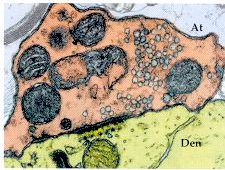
\includegraphics[width=0.1\textwidth]{images/dendrite.png}
        };

        \node[image] (n3) at ([xshift=\shifty,yshift=-1cm]mm) {
            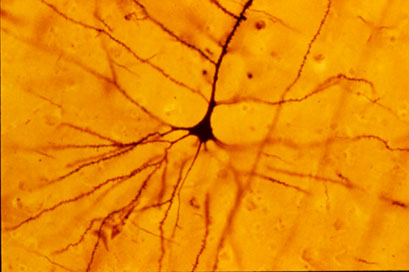
\includegraphics[width=0.1\textwidth]{images/GolgiStainedPyramidalCell.jpg}
        };

        \node[image] (n5) at ([xshift=\shifty,yshift=-1.0cm]m) {
            \includegraphics[width=0.1\textwidth]{images/brain.png}
        };

        \node[image] (n4) at ([xshift=\shifty,yshift=1cm]mm) {
            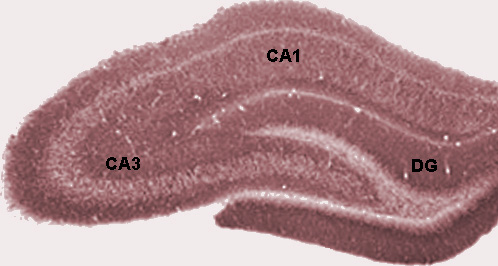
\includegraphics[width=0.1\textwidth]{images/HippocampalRegions.jpg}
        };


        \node[rectangle, minimum width=12cm, minimum height=6.0cm,
            draw, rounded corners] (chemical) at (9.0,4.5) {};

        \node[] (caption) at ([yshift=-1cm]chemical.north) {\LARGE Chemical};

        \node[rectangle, minimum width=3cm, minimum height=4.5cm
            , draw, rounded corners
            ] (electrical) at (3.5, 9.0) {};

        \node[] at (electrical.center) {\LARGE Electrical};


        % Put chemical network here
        \node[] (network) at (7.0,4.0) {
            \includegraphics[width=5cm]{images/chemical_reactions.png}
        };

        \node[] (chromosome) at (12.0,5) {
            
\includegraphics[width=5cm]{images/chromosome.png}
        };

        \node[] (text) at ([xshift=5cm,yshift=4cm]electrical.east) {
            \begin{minipage}{0.3\textwidth}
                \LARGE\bf
                \begin{itemize}
                    \item $10^{11}$ cells, $10^{15}$ synapses, $10000$? reactions per synapse
                    \item Electrical events: $< 1$ ms,  Chemical events: $1\;
                        \text{sec} \rightarrow 1000\; \text{sec}$
                \item Structural events: $100\; \text{sec} \rightarrow \text{months}$
        \end{itemize}
    \end{minipage}
};
    \end{tikzpicture} %
    \begin{tikzpicture}
        \node[] (stochastic) {
            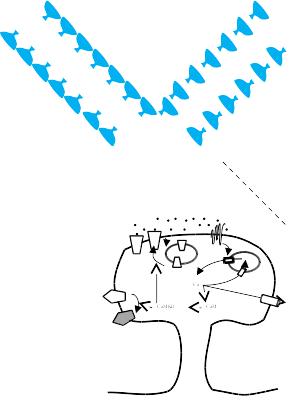
\includegraphics[width=\figwidth]{./images/stochastic_solver.png}
        }; 
        \node[text width=1.5*\figwidth] at ([xshift=2.5cm]stochastic.east)
        {\CAPTION{Reaction at single molecule level}};
        \node[] (ksolve) at ([yshift=-2cm]stochastic.south) {
            \includegraphics[width=\figwidth]{./images/ksolve_dsolve.png}
        };
        \node[text width=1.5*\figwidth] at ([xshift=2.5cm]ksolve.east) {\CAPTION{Reaction Diffusion Solver}};
        \node[] (hsolve) at ([yshift=-2cm]ksolve.south) {
            \includegraphics[width=\figwidth]{./images/hsolve.png}
        };
        \node[text width=1.5*\figwidth] at ([xshift=2.5cm]hsolve.east)
        {\CAPTION{Electrical: Hines Solver}};
    \end{tikzpicture}
    \end{Figure}

    \begin{Figure}
        \edef\figwidth{0.3\columnwidth}
        \begin{tikzpicture}
            \node[] (signalling)  {
                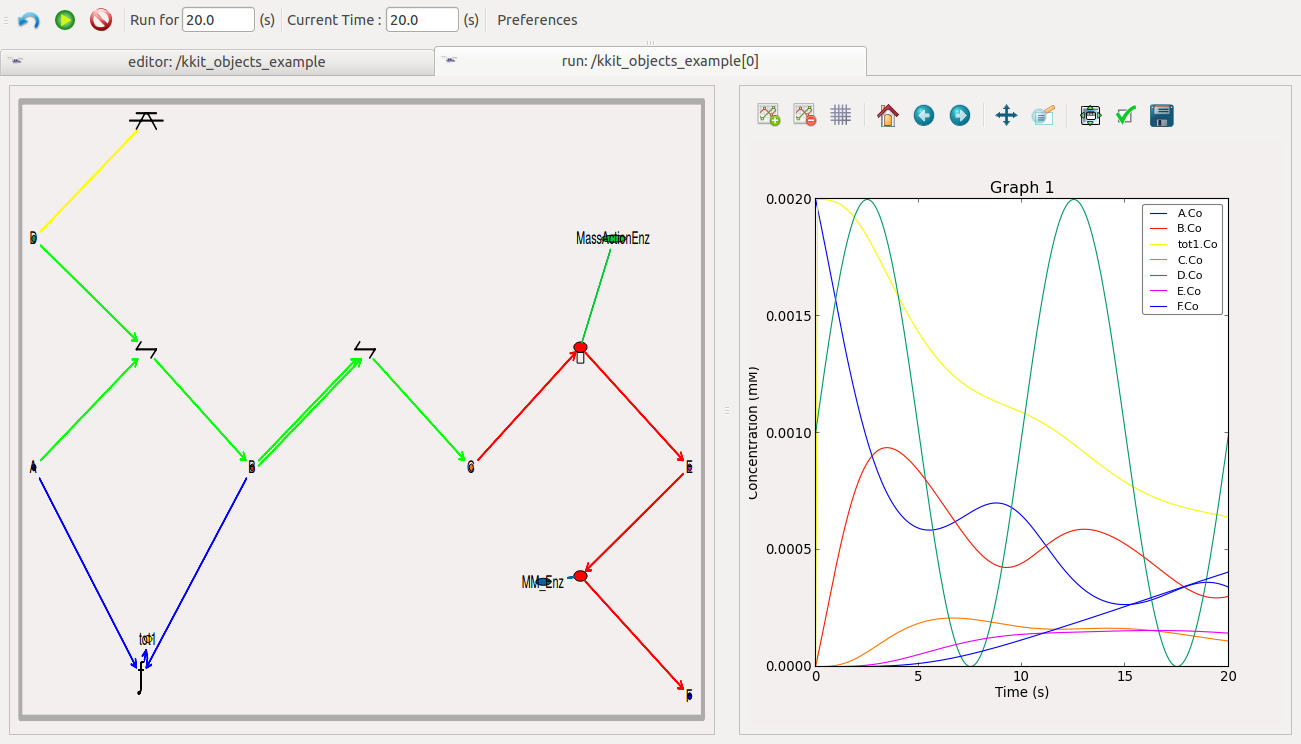
\includegraphics[width=\figwidth]{./images/poster_runView.png}
            };
            \node [text width=\figwidth, below=2.7cm] (captionC)  {\CAPTION{Signalling Model}};
        \end{tikzpicture}%
        \begin{tikzpicture}
            \node [] (moose_cell) {
                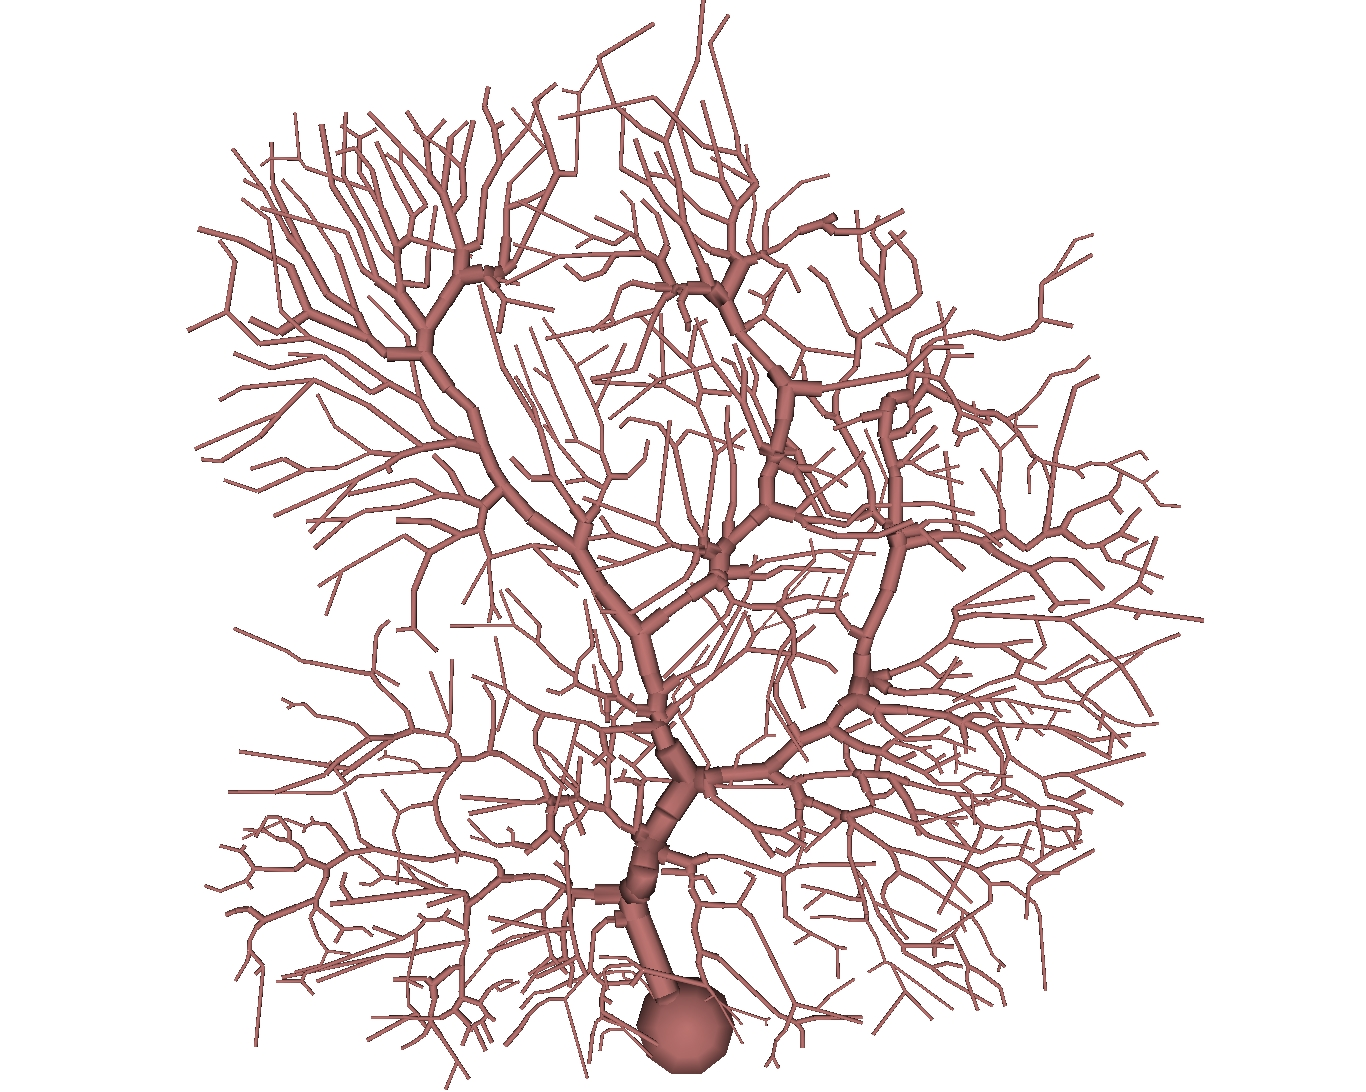
\includegraphics[width=\figwidth]{./images/_1_7.jpeg}
            };
            \node [text width=\figwidth,below=3.5cm] (captionA) {\CAPTION{Single Neuron Model}};
        \end{tikzpicture}%
        \begin{tikzpicture}
            \node[] (olfaction) {
                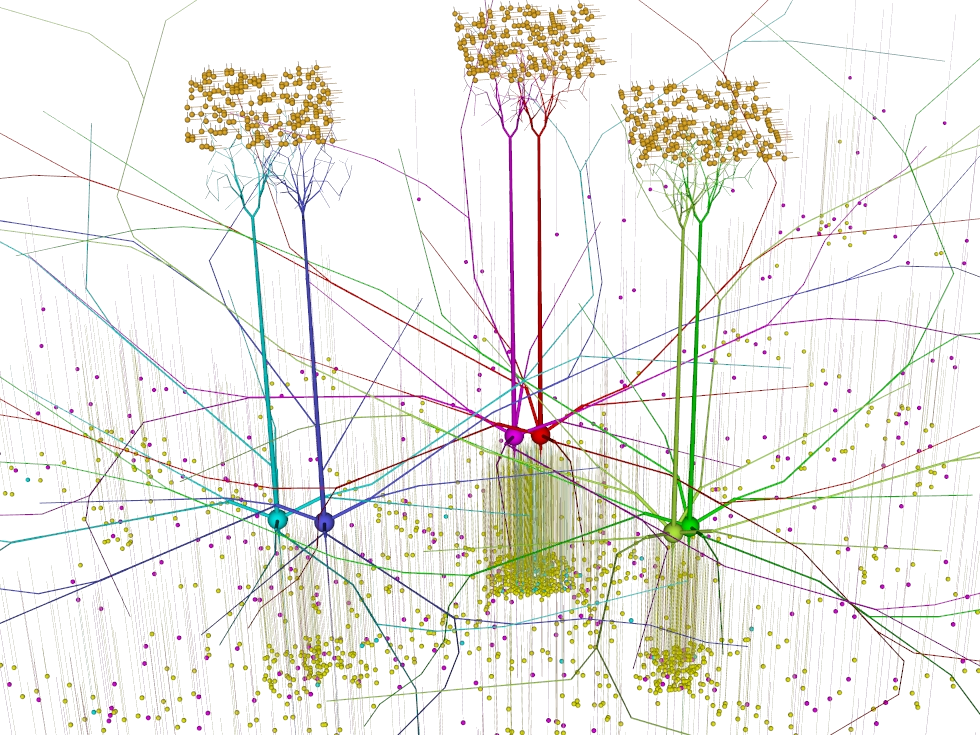
\includegraphics[width=\figwidth]{./images/fullmodel_moogli.png}
            };
            \node [text width=\figwidth, below=2.7cm] (captionB) {\CAPTION{Olfactory
                    bulb model}};
        \end{tikzpicture}
\end{Figure}
\vfill
\columnbreak

\HEADING{Some projects using \MOOSE}
\begin{Figure}
    \edef\figwidth{0.9\textwidth}
    \begin{tikzpicture}
        \node[fill=red!3] (aditya) {
            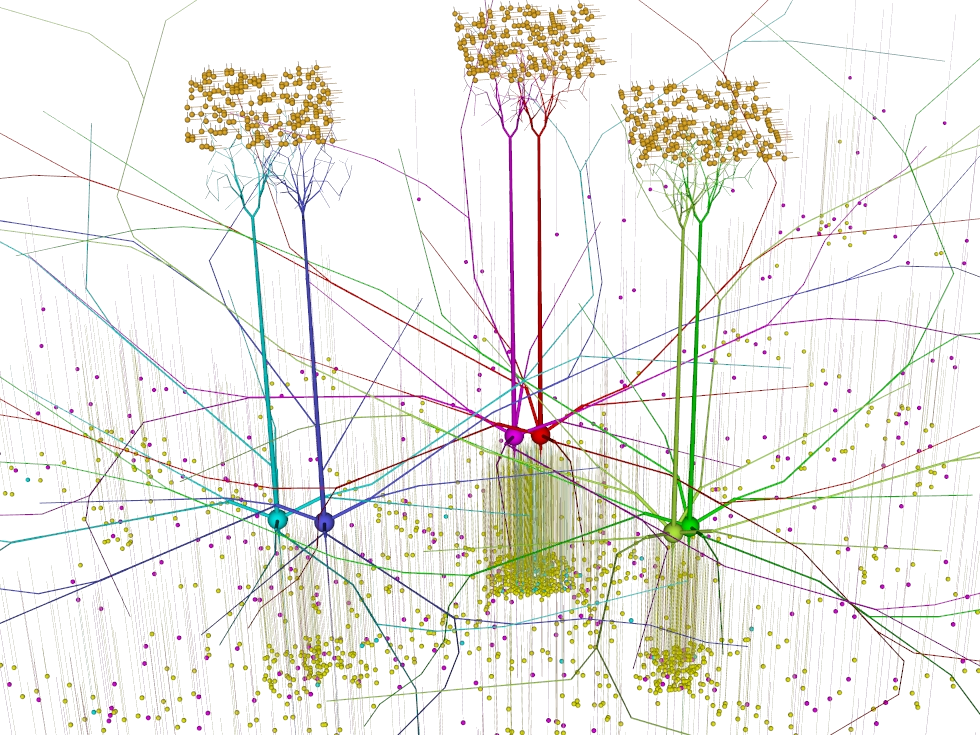
\includegraphics[width=\figwidth]{./images/fullmodel_moogli.png}
        };
        \node [] (result) at ([yshift=-2cm]aditya.south) {
            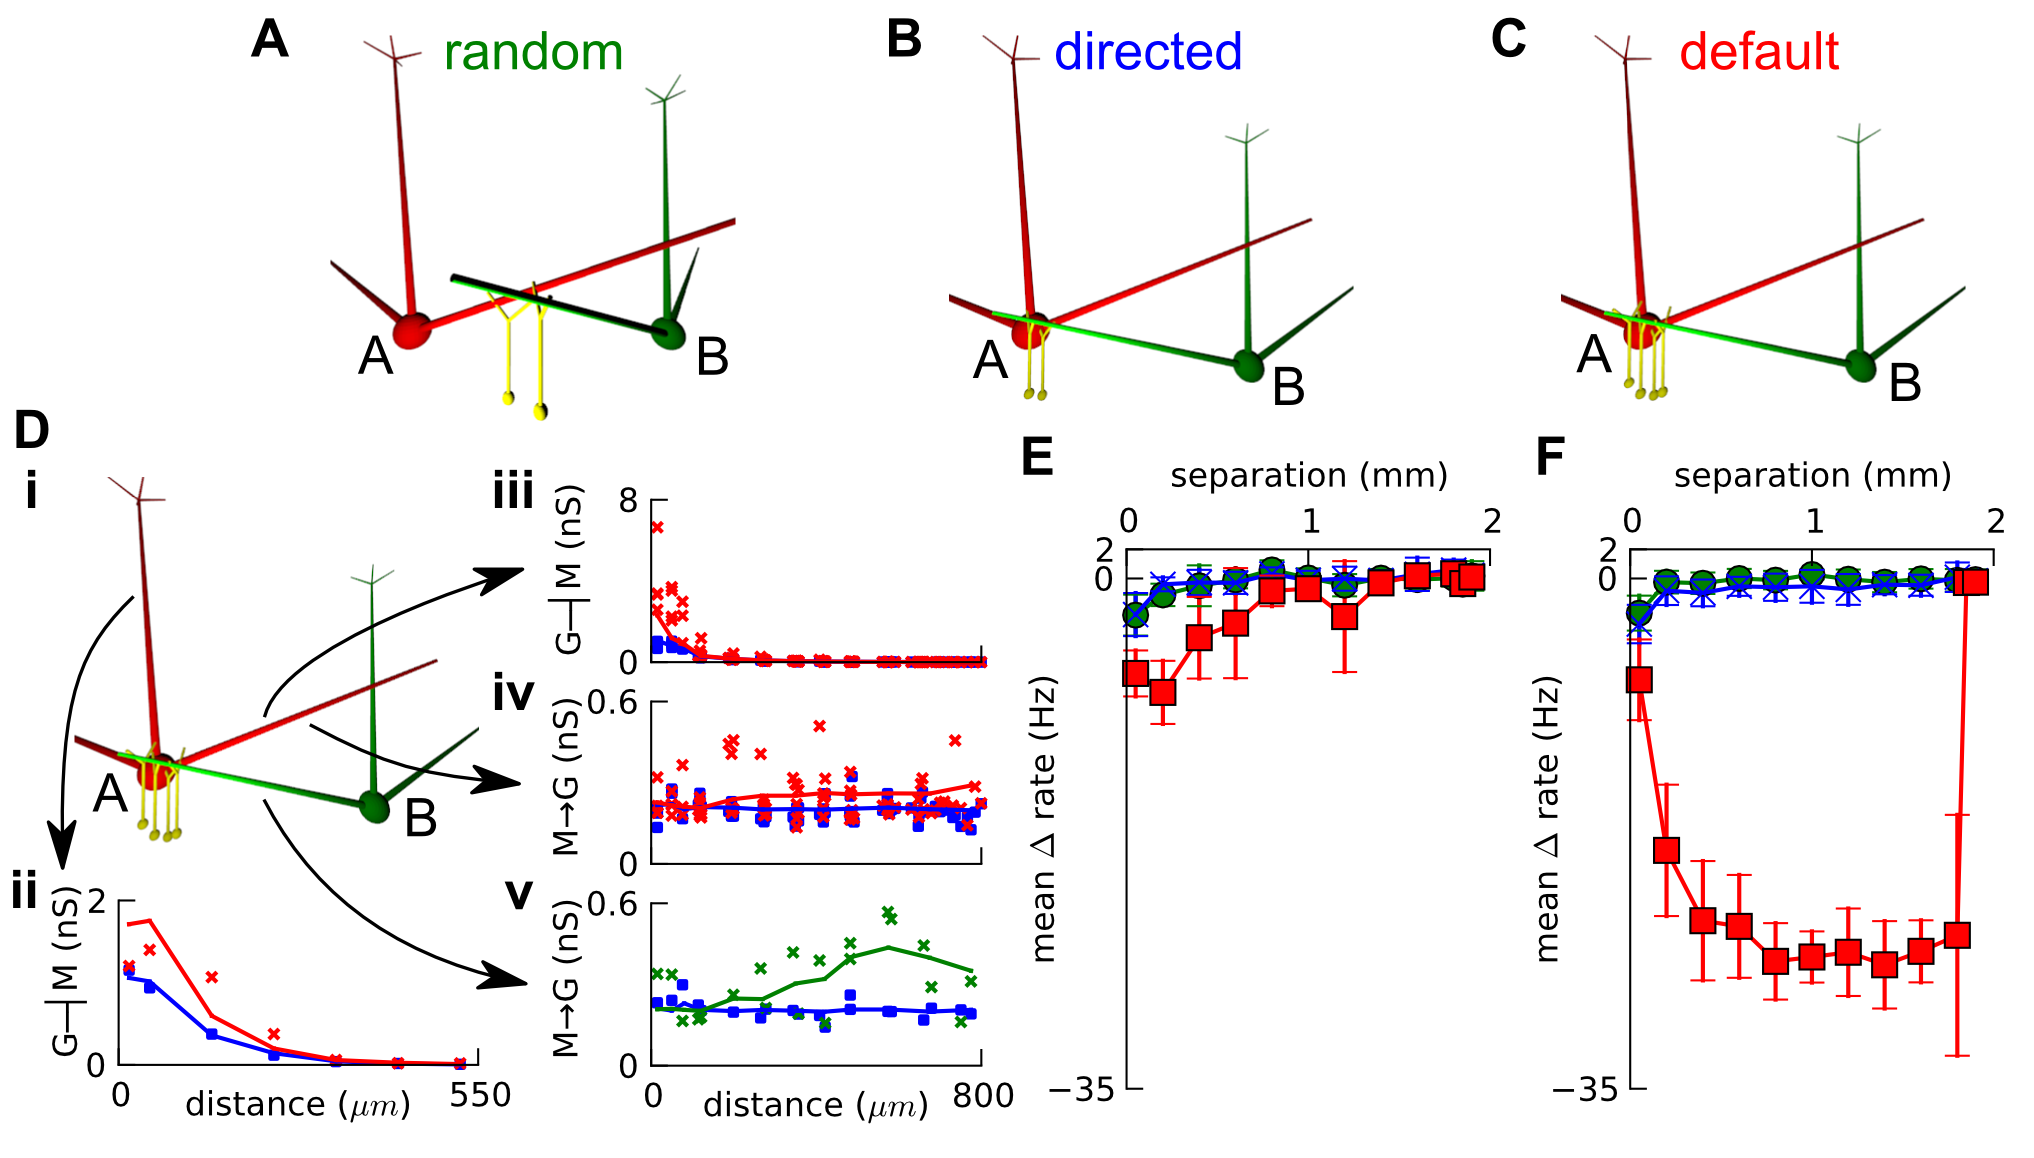
\includegraphics[width=\figwidth,trim=0cm 0cm 0cm 3.4cm, clip]{./images/aditya_work.png}
        };

        \node[minimum height=0cm,text width=\figwidth] (aditya_caption) at
        ([yshift=-1cm]result.south) {
            \CAPTION{ Network coding and computation in olfaction and sematosensory
                cortex. It explains linear coding and phase-decorrelation and
                predicts connectivity, lateral dendrite output structure.
            }
        };
    \end{tikzpicture}
    %% One more model here.

    \begin{tikzpicture}
        \node[] (robust) {
            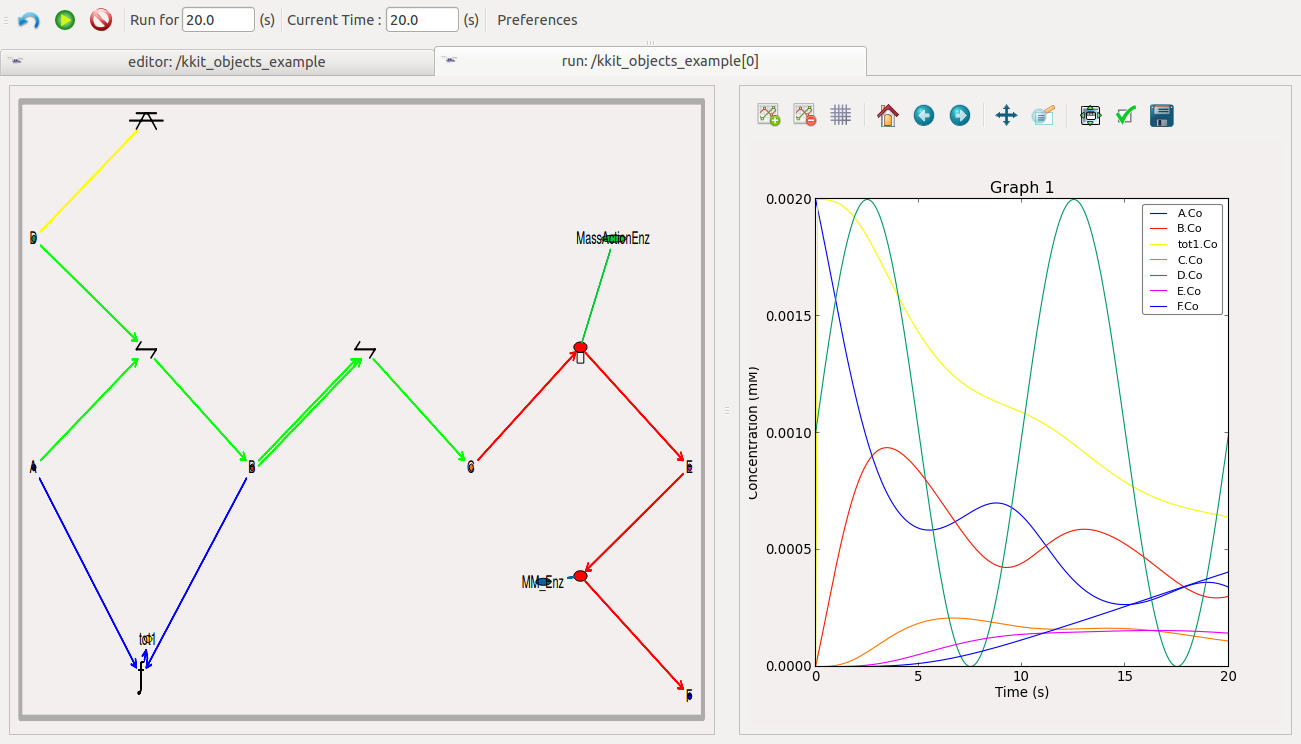
\includegraphics[width=\figwidth]{./images/poster_runView.png}
        };

        \node[text width=\figwidth] at (robust.south) {
            \CAPTION{Robustness of chemical switches with respect to stochasticity and parameters.}
        };

    \end{tikzpicture}
\end{Figure}

%% Column 3
\begin{Figure}
    
    \HEADING{Sahil}

    \begin{tikzpicture}
        \node [] (timeseries) {
            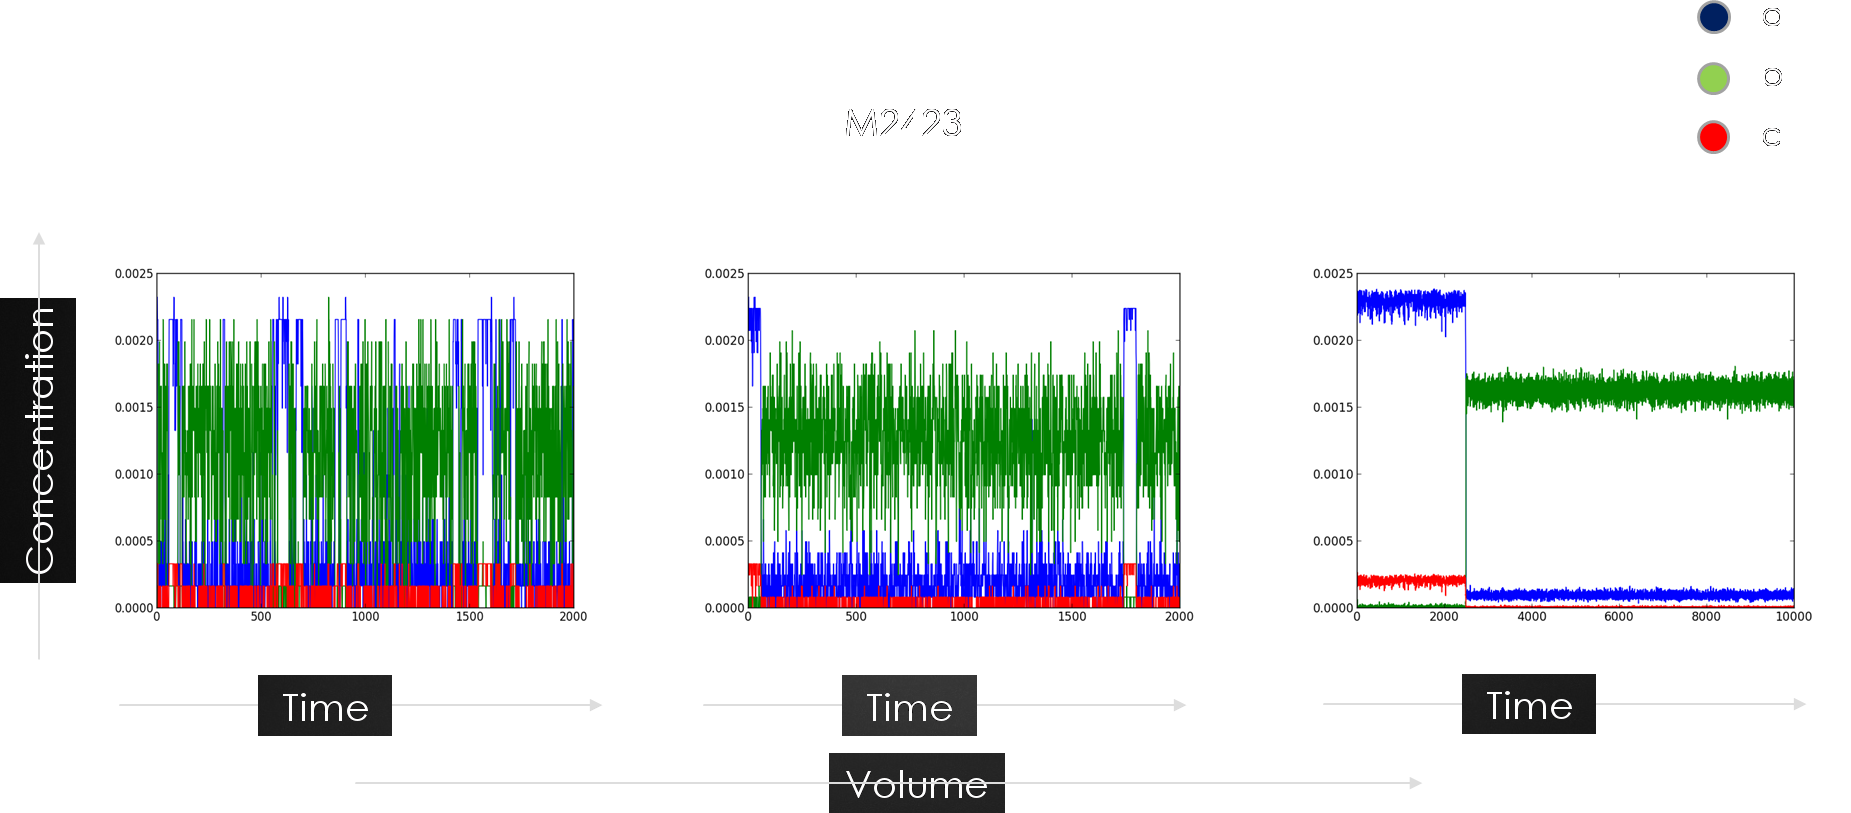
\includegraphics[width=0.9\textwidth]{./images/TimeSeries.png}
        };
    \end{tikzpicture}

    \begin{tikzpicture}
        \node [] (timeline) {
            \includegraphics[width=0.9\textwidth]{./images/timeline.png}
        };
    \end{tikzpicture}

    \begin{tikzpicture}
        \node [] (model) {
            \includegraphics[width=0.45\textwidth]{./images/model.png}
        };
    \end{tikzpicture}%
    \begin{tikzpicture}
        \node[] (ktseries) {
            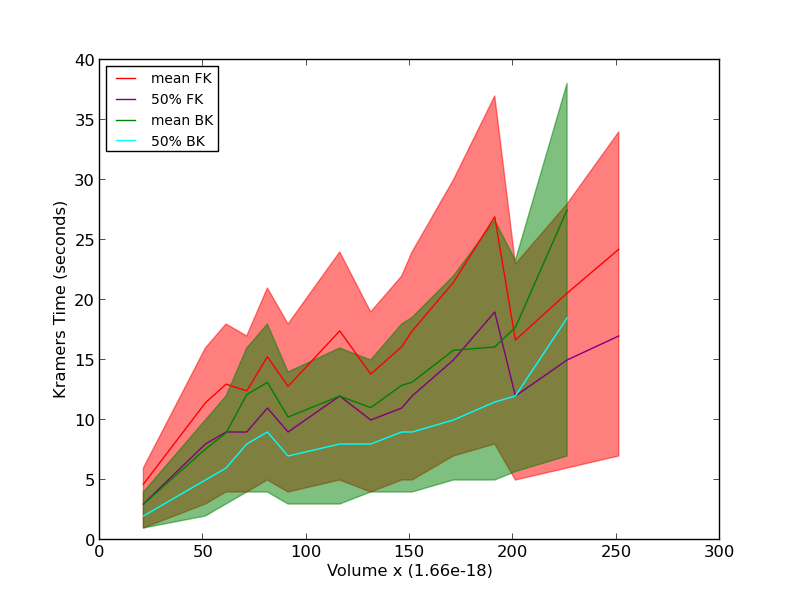
\includegraphics[width=0.45\textwidth]{./images/KT_statistic.png}
        };
    \end{tikzpicture}

    \HEADING{Summary}
    \HUGE We use models to
    \begin{itemize}
            
        \item Integrate many scales of neuronal data with basic
            physical/chemical principles.
        \item Explain phenomenon of plasticity, activity and neuronal coding.
        \item Predict circuit mechanisms, plasticity rules, and emergent
            phenomena such as \emph{decorrelation}, \emph{robustness}, and
            \emph{memory decay}.

    \end{itemize}

    \textbf{We have developed MOOSE to carry out these simulations}.

\end{Figure}

\end{multicols}

\end{document}
